\begin{figure}[p]
\centering
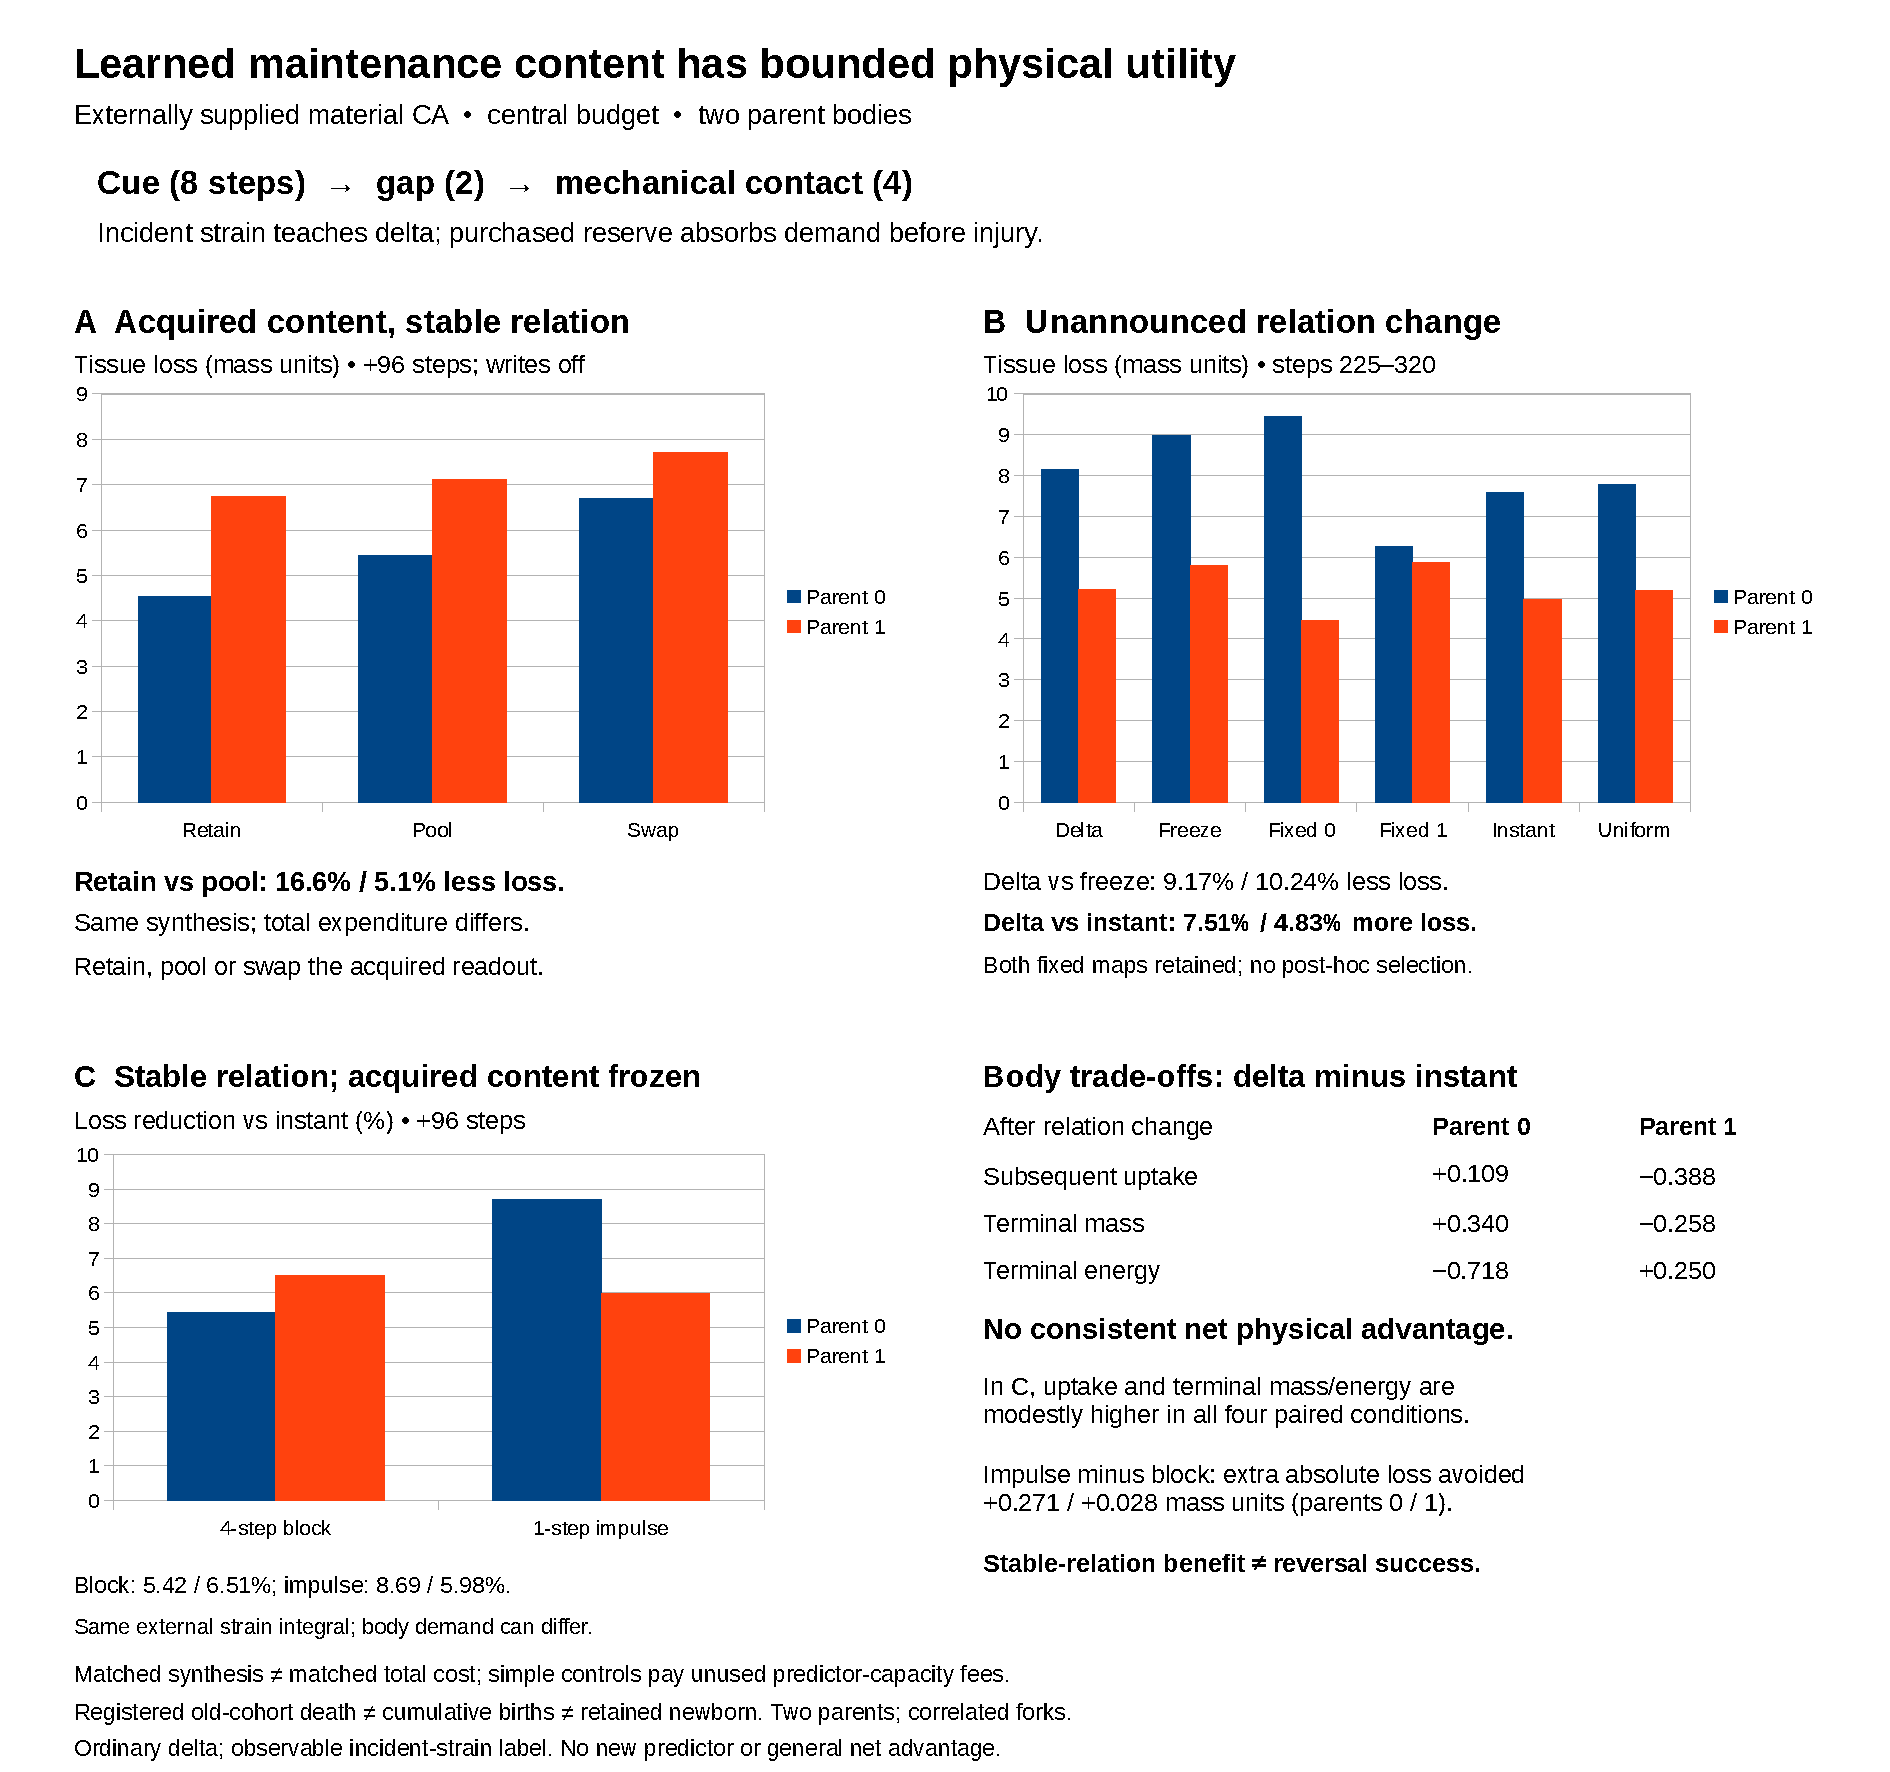
\includegraphics[width=\linewidth,height=0.63\textheight,keepaspectratio]{work/longform_v047/figures/predictive_maintenance_v048/predictive_maintenance.pdf}
\captionsetup{font=footnotesize}
\caption{\textbf{Acquired conditional maintenance has limited physical utility against strong instantaneous controls.}
The externally supplied, density-regulated material CA has centrally coordinated purchasing and a local incident-strain sensor. The ordinary conditional delta rule learns from completed contact, including strain absorbed by reserve; it is not a new predictor.
\textbf{a}, All three content readouts of two acquired parents over 96 new steps with writes stopped and the learned relation retained. Retaining rather than pooling content reduces injury by 16.6\%/5.1\% at equal realized reserve synthesis; swapping also raises injury.
\textbf{b}, All six policies from both actual parents. Bars show injury in steps 225--320 after the relation changes at boundary 224. Continued delta reduces injury relative to frozen content by 9.17\%/10.24\%, but loses 7.51\%/4.83\% more tissue than the instantaneous rule. Neither fixed map is selected retrospectively. The accompanying delta-minus-instantaneous contrasts show opposed uptake and terminal mass/energy effects, without consistent net benefit.
\textbf{c}, Two actual 192-step parents each supply four 96-step futures under the retained relation, crossing block/impulse contact with acquired/instantaneous readout; writes are frozen. External strain integrals match, while realized bodily demand can differ. Bars show paired injury reductions relative to instantaneous allocation. The impulse increases the absolute avoided-loss contrast by 0.271/0.028 mass units, but proportional benefit does not rise in both parents. This is a stable-relation expression test, not reversal success or isolation of one timing mediator.
Colours identify source parents within each assay; their branches are correlated conditions. Equal synthesis does not equalize total expenditure. Simple controls carry unused predictor capacity and its fees. Old-cohort death, cumulative birth and retained newborn tissue are distinct; none establishes newborn-content necessity. The original missing risk tail is not imputed. Full phase outcomes and physical accounts are in the accompanying maintenance source tables.}
\label{fig:predictive-maintenance}
\end{figure}
